%这是LaTeX源文件
%编译要求:
%编译命令: xelatex -shell-escape rep.tex
%其他要求: 需要安装字体Bitstream Vera Sans Mono;需要安装pygments;需要文档类'cumtbrep';需要实验中用到的代码文件

\documentclass{cumtbrep}

\usepackage{float}
\usepackage{graphicx}
\usepackage{amsmath}
\usepackage{upgreek}
%hyper ref
\usepackage{hyperref}
\hypersetup{colorlinks,bookmarks=false,pdfauthor=王凌峰,pdftitle=报告7}
%font spec
\usepackage{fontspec}
\newfontfamily\bvsm{Bitstream Vera Sans Mono}[NFSSFamily=bvsmfamily]
%code
\usepackage{listings}
\usepackage{minted}
\setminted{breaklines,breakanywhere,mathescape,tabsize=4,style=default,fontsize=\normalsize,fontfamily=bvsmfamily,linenos}
%codes' line number format
\renewcommand{\theFancyVerbLine}{\sffamily
\textcolor[rgb]{0.5,0.5,0.5}{\scriptsize\oldstylenums{\arabic{FancyVerbLine}}}}
%listing's caption
\usepackage{caption}
\captionsetup{tablename=code}
%code with caption
\newcommand\inputcode[3][c++]{%
	\inputminted{#1}{#2}
	\begin{figure}[H]
		\centering
		\captionsetup{type=table}
		\caption{\texttt{#3}}
	\end{figure}
}
\newcommand\inline[2][c++]{\mintinline{#1}{#2}}

\begin{document}

\makeheader{计算机图形学}{王振武}{计科\numberstyle 19-2}{王凌峰}{\numberstyle 1910630221}

\namesec
\begin{enumerate}
	\setcounter{enumi}{6}
	\item 纹理映射
\end{enumerate}

\purposesec
\noindent 完成纹理映射

\contentsec
把\hyperref[fig:wall]{某种墙的纹理}映射到球面上。

实际上OpenGL的纹理映射是在rasterization过程中发生的,rasterization阶段产生的fragments被送入fragment shader处理,像素的颜色也在此阶段决定。因此和实验1~实验3一样,这里也只是纹理映射的模拟。

目录结构:{\ttfamily \lstinputlisting{../texture/tree}}

为了获得与每个点关联的颜色,fragment shader中声明 \inline[glsl]{in vec3 texColor},颜色直接从 \inline[glsl]{texColor} 中取出:
\inputcode[glsl]{../texture/trivial.frag}{trivial.frag}

fragment shader的变量 \inline[glsl]{texColor} 由vertex shader传入:
\inputcode[glsl]{../texture/trivial.vert}{trivial.vert}

图片 \path{wall.jpg} 的读取用 \inline{stb} 库。该库是header-only library,其要求存在一个 \path{.cc} 文件包含 \inline{stb} 库相应头文件的实际实现:
\inputcode{../texture/image.cc}{image.cc}

这个实验使用了 \inline{point} 和 \inline{rgb} 类,其中 \inline{point} 类与之前实验的类似,只是扩展到了三维:
\inputcode{../texture/point.hh}{point.hh}
\inputcode{../texture/point.cc}{point.cc}

\inline{rgb} 类只是颜色分量的集合:
\inputcode{../texture/rgb.hh}{rgb.hh}
\inputcode{../texture/rgb.cc}{rgb.cc}

\inline{rasterize_with_texture} 将球心坐标$\vec o$,半径$300$的球体rasterize,并根据每个像素的位置$(\varphi,\theta)$映射到纹理图片,取出相应颜色与该像素绑定,返回所有像素点及与其对应的颜色。

\path{texture.cc} 中用的是粗糙的rasterization的方法。对$\varphi \in [0,2\uppi]$及$\theta \in [0,\uppi]$分别以某个步长遍历,得到整个球面上采样点的坐标。步长越小,球面就显示得越精细。这个实验中$\Delta\theta$和$\Delta\varphi$都为$0.2^\circ$,效果可以接受。

图片上点的自由度为2,球面上点的自由度也是2,可以方便地建立映射。为了更方便,使用$\mathit{row}=A\cdot\theta+C_1,\mathit{col}=B\cdot\varphi+C_2$的形式。

令$C_1=C_2=0,A\cdot\theta_{\mathit{max}}=\mathit{height},B\cdot\frac{1}{2}\cdot\varphi_{\mathit{max}}=\mathit{width}$,其中$\mathit{width}$和$\mathit{height}$分别为纹理图片以像素为单位的宽度和高度。则每半个球面分布一张纹理图片。
\inputcode{../texture/texture.hh}{texture.hh}
\inputcode{../texture/texture.cc}{texture.cc}

camera transformation与三维图形变换实验中用到的类似,以$\vec o$为圆心在$xOz$平面上以半径$400$绕$y$轴旋转。
\inputcode{../texture/main.cc}{main.cc}

\analysesec
\begin{figure}\label{fig:wall}
	\centering
	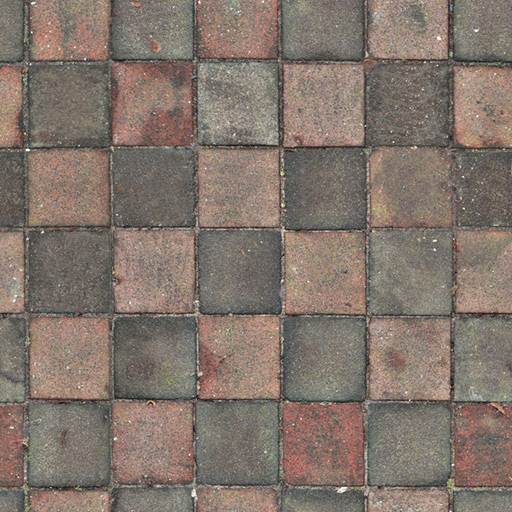
\includegraphics[scale=0.4]{../texture/wall.jpg}
	\caption{某种墙的纹理}
\end{figure}
\begin{figure}
	\centering
	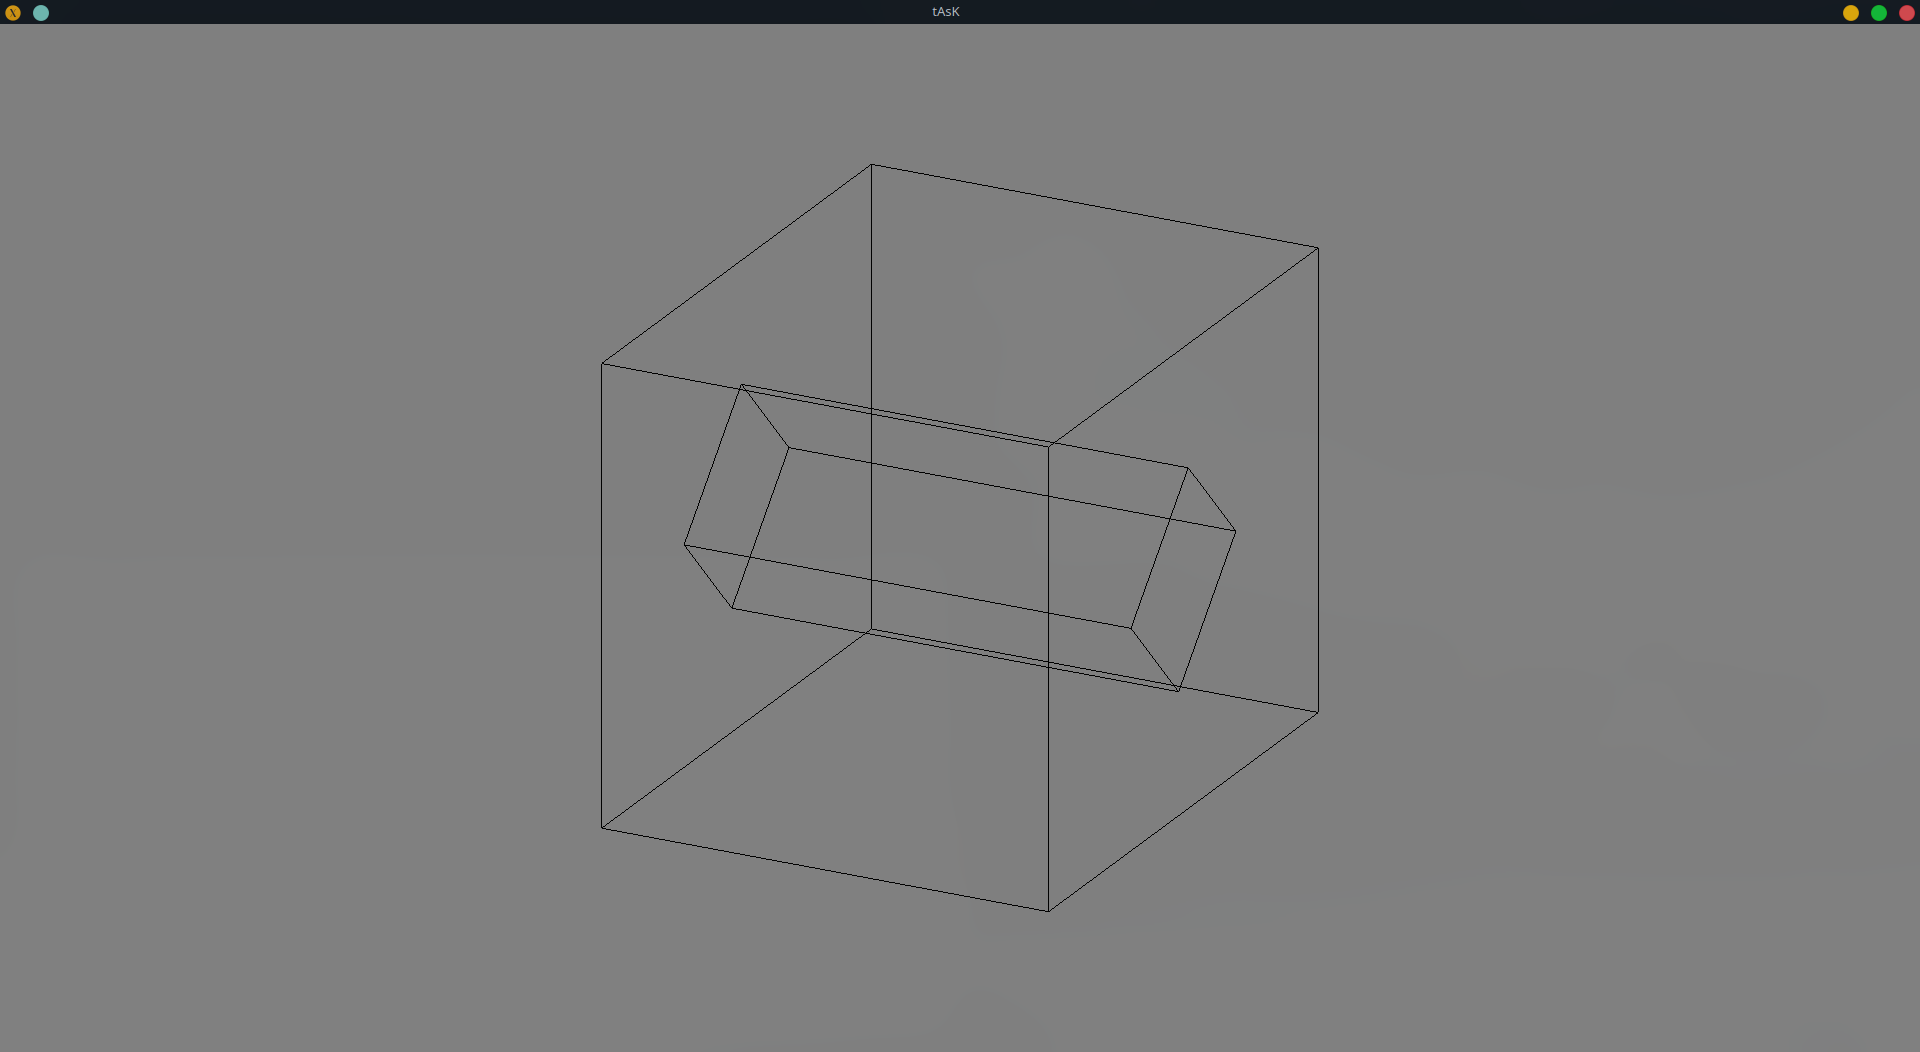
\includegraphics[scale=0.3]{../texture/1.png}
	\caption{效果}
\end{figure}
\begin{figure}
	\centering
	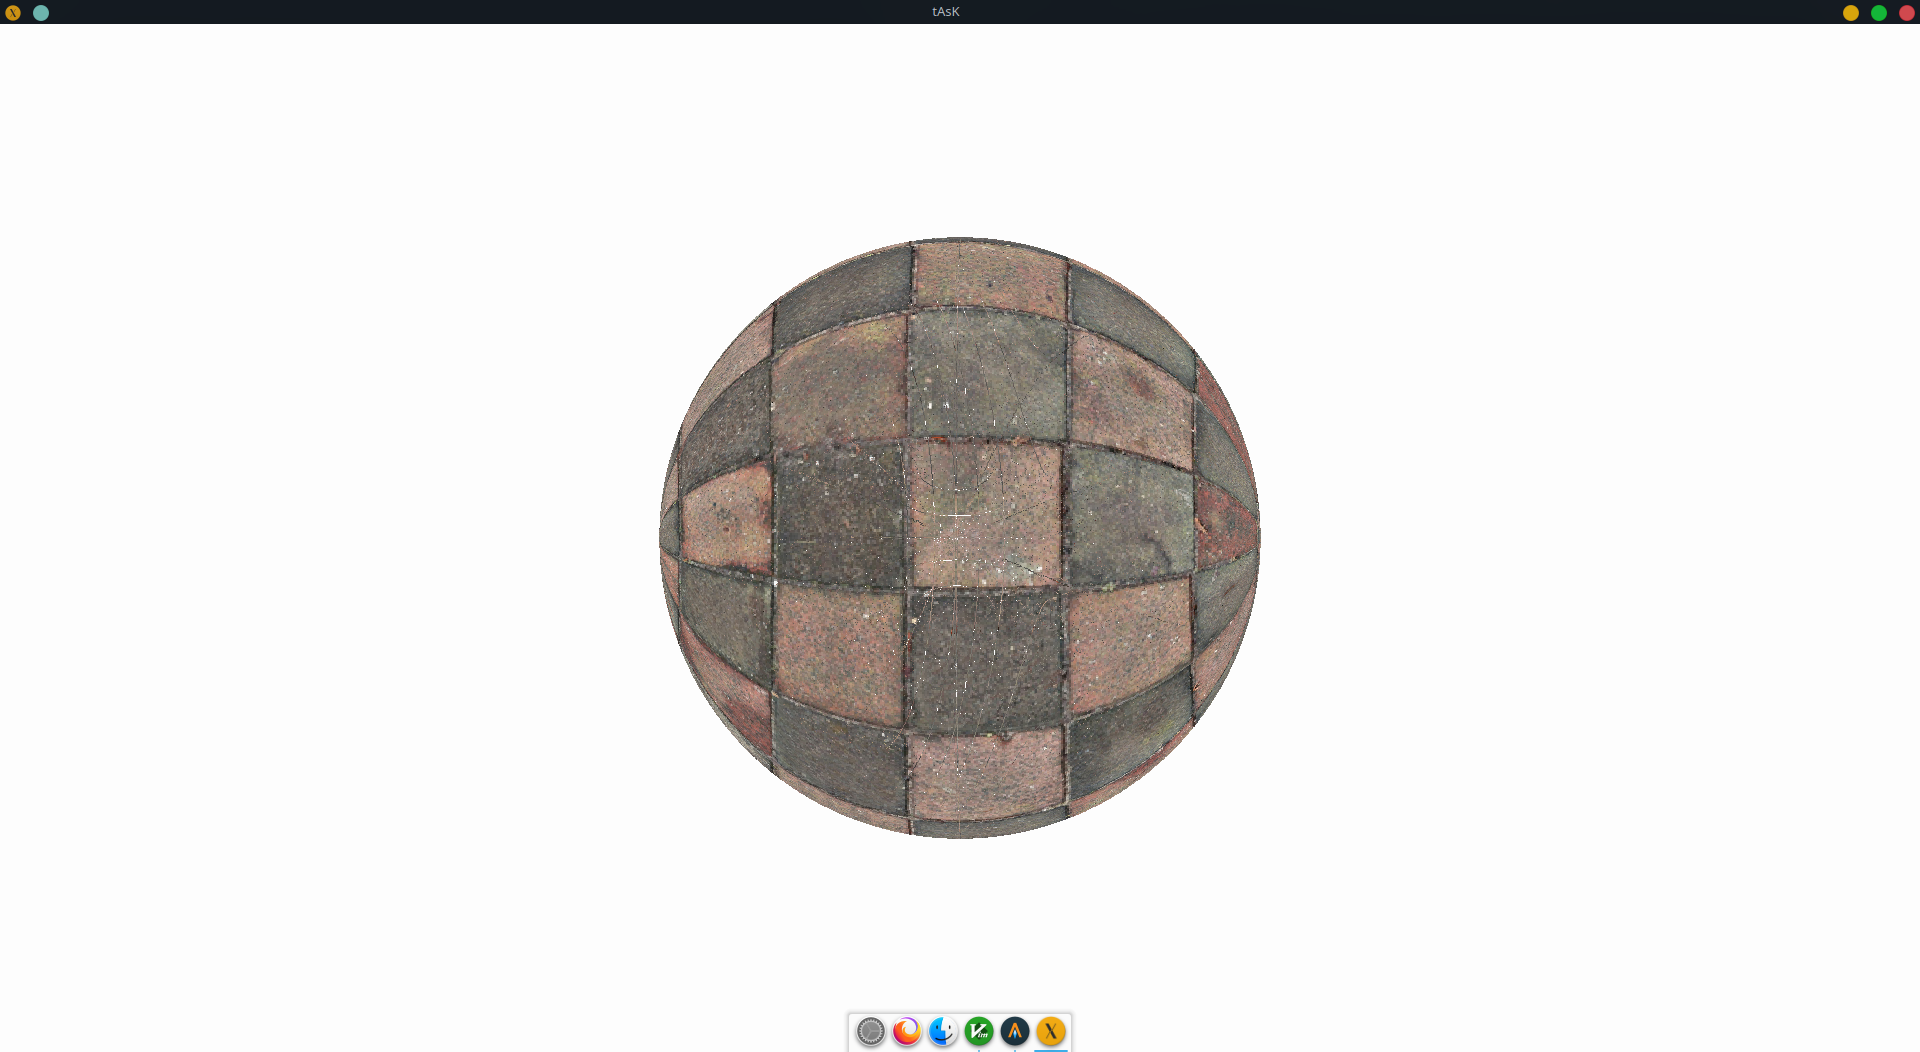
\includegraphics[scale=0.3]{../texture/2.png}
	\caption{另一个角度的效果}
\end{figure}

\maketail

\end{document}
